\chapter{Définitions}
\label{ch:Ch1}

%%%%%%%%%%%%%%%%%%%%%%%%%%%%%%%%%%%% SECTION 1
\section{\textbf{$X_{T}$}}
\label{sec:Ch1.1} 

le point d'application d'un effort est une notion importante. Si celui de l'effort aérodynamique et du poids sont couramment utilisés, le point d'application de la tension des lignes influence beaucoup les performances d'un kite. De plus, le bridage d'un kite change considérablement la façon dont se répartie la tension dans les lignes et l'angle d'équilibre au zénith d'un kite. Ainsi, afin de capturer l'influence du bridage sur les performances d'un kite, on définit $X_T$ comme étant \textbf{le point d'intersection entre la corde moyenne d'un kite et l'axe de la tension des lignes; ce dernier étant tangant au dernier segment des lignes}. Ainsi, $X_T$ permet de lié la géométrie du bridage et son influence sur la dynamique du kite.  \\

\begin{figure}[H]
    \centering
    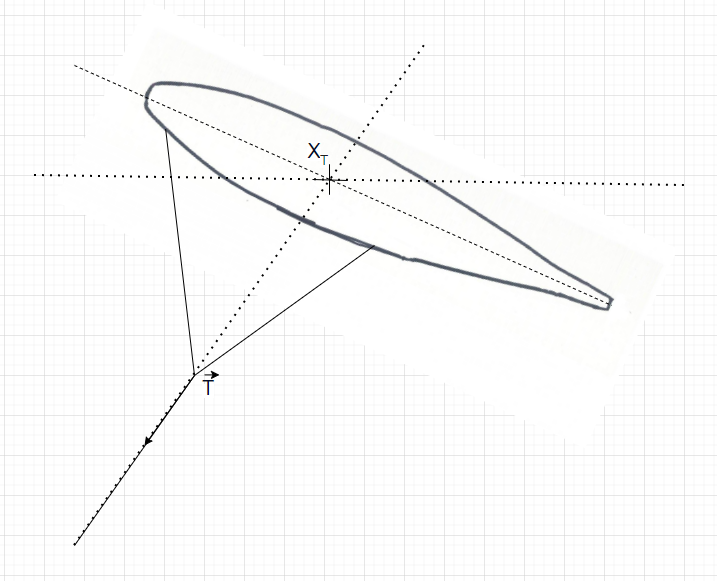
\includegraphics[width=0.5\textwidth]{Pics/01 - Définitions/Xt.png}  
    \caption{Xt}
    \label{fig:Xt}
\end{figure}

Isoler les ensembles \{kite\} et \{kite+bridage\} permet de montrer $X_T$ est le point d'application de l'ensemble du bridage, le long de la corde. En effet :

Pour l'équilibre des moments appliqué à l'ensemble \{kite\}, en le $X_T$ :
\begin{equation}
    F_{Poid}(x_G-x_T)+F{aero}(x_{aero}-x_T) = 0
\end{equation}

Pour l'équilibre des moments appliqué à l'ensemble \{kite+bridage\}, $X_T$:
\begin{equation}
    F_{Poid}(x_G-x_T) + F{aero}(x_{aero}-x_T) + \sum_{i=A}^{D} F_{ligne i}(x_{ligne i}-x_T)= 0
\end{equation}

D'où : 
\begin{equation}
    \sum_{i=A}^{D} F_{ligne i}(x_{ligne i}-x_T)= 0
\end{equation}

Ce qui, par définition, montre que \textbf{$X_T$ est le point d'application de la résultante de tension de l'ensemble du bridage projeté sur la corde.}

%%%%%%%%%%%%%%%%%%%%%%%%%%%%%%%%%%%% SECTION 2
\section{\textbf{Tow Point}}
\label{sec:Ch1.2} 

On définit le Tow Point par \textbf{le projeté orthogonal du point d'attache entre les lignes et le bridage sur la corde moyenne du kite}. 

\begin{figure}[H]
    \centering
    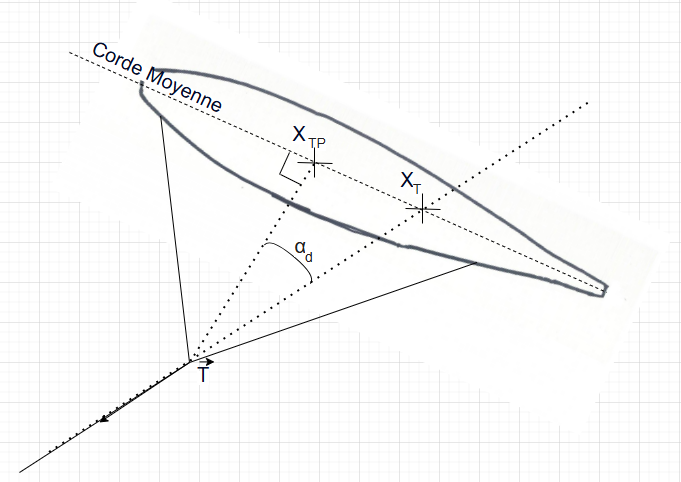
\includegraphics[width=0.5\textwidth]{Pics/01 - Définitions/xtp.png}  
    \caption{Différence entre $x_{TP}$ et $x_T$}
    \label{fig:Xtp}
\end{figure}

Le schéma \ref{fig:Xtp} montre que le towpoint ($x_{TP}$) et $x_T$ forment un angle $\alpha_d$, \textbf{l'angle de depower}, avec le point d'attache entre les lignes et le bridage. Ainsi, dans le cas où les lignes forment un angle de $\frac{\pi}{2}$ avec la corde moyenne du kite, Tow Point et $x_T$ sont confondus. 

De plus, $x_{TP}$ est purement géométrique là où $x_T$ lie géométrie et aérodynamique.

On peut lier ces deux positions par la relation suivante : 

\begin{equation}
    x_{TP} = x_T + d * tan(\alpha_d)
    \label{eq:Xtp}
\end{equation}

où d est la distance du point d’attache entre les lignes et le bridage à la corde moyenne, divisé par la corde profil.

%%%%%%%%%%%%%%%%%%%%%%%%%%%%%%%%%%%% SECTION 3
\section{Comparaison avec la littérature}
\label{sec:Ch1.3} 

En comparaison avec le papier de Fechner (2015) intiltulé "Dynamic Model of a Pumping Kite Power System", l'angle $\alpha_d$ tel que nous le définissons ici est lié à celui définit par ce papier par la relation $\alpha_d = -(\alpha_{d, Fechner} + \alpha_0)$ : 

\begin{figure}[H]
    \centering
    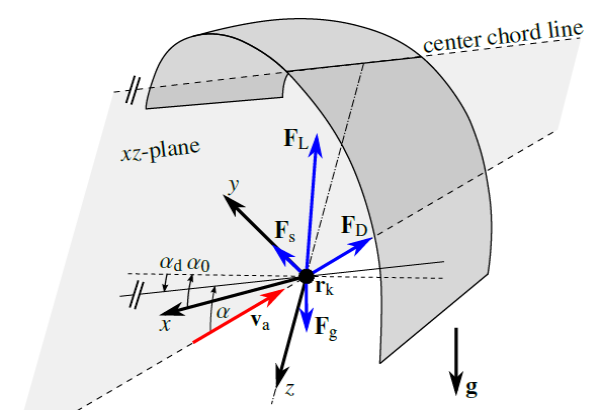
\includegraphics[width=0.5\textwidth]{Pics/01 - Définitions/fechner alpha d.png}  
    \caption{Présentation des angles du kite}
    \label{fig:fechner alpha d}
\end{figure}

Ce papier choisit de définir $\alpha_0$ comme étant l'angle que fait la corde moyenne du kite par rapport à l'orthogonal des lignes dans la direction du vent (axe ($r_x$, $\overrightarrow{e_x}$)) quand la barre est bordée au maximum, et suppose donc ainsi que cet angle est constant. Or selon le vent relatif le fardage des lignes change, et ainsi $\alpha_0$ n'est pas rigoureusement constant car $X_T$ (définit en \ref{subsec:Ch1.1.1}) se déplace alors le long de la corde.\\

Rigoureusement, on devrait écrire $\alpha_0(v_{wind})$, car l'équilibre statique du kite dépend du vent réel...\\

Nous décidons donc ici de définir $\alpha_d$ par rapport aux axes liés au système. Cela permet d'avoir des angles pertinants pour la dynamique du vol et la dynamiques des fluides autour du kite, et dont la valeurs dépend de l'état du système. 

La figure \ref{fig:fechner alpha d} fait le choix d'un repère aligné avec le dernier segment des lignes ( i.e. aligné avec la tension des lignes et passant par le point d'attache avec le kite), orienté dans la direction du vent relatif. Ce repère est pertinant pour nos études. 

%%%%%%%%%%%%%%%%%%%%%%%%%%%%%%%%%%%% SECTION 4
\section{Conclusion sur les définitions}
\label{sec:Ch1.4}

Cette sous partie a permit de montrer la difficulté à définir les différentes grandeurs qui gravitent autour d'un kite, ainsi que leur dépendances aux conditions aérologique. Nous avons ainsi définit :
\begin{itemize}
    \item \textbf{$X_{TP}$ / Tow Point} : le Tow Point est le projeté orthogonal du point d’attache entre les lignes et le bridage sur la corde moyenne du kite (Cf \ref{sec:Ch1.2})
    \item \textbf{$X_T$} : ce point est le point d’intersection entre la corde moyenne d’un kite et l’axe de la tension des lignes en le point d'attache; cet axe/effort étant tangant au dernier segment des lignes, il dépend du fardage et donc de $v_{wind}$. Aussi, $X_T$ est le point d’application de la résultante de tension de l’ensemble du bridage projeté sur la corde (Cf \ref{sec:Ch1.2})
    \item \textbf{$\alpha_d$} : $\alpha_d$ est \textbf{l'angle de depower}. C'est l'angle que forment le towpoint et $X_T$ avec le point d'attache entre les lignes et le bridage (Cf la figure \ref{fig:Xtp}). Il est aussi l'angle entre la corde moyenne du kite et l'orthogonal au dernier segment de ligne dans l'alignement du vent relatif (Cf \ref{sec:Ch1.3}). cette angle \textbf{dépend des conditions aérodynamiques ($v_{wind}$, équilibre, ...)}puisqu'il dépend de $X_T$, donc de la tension des lignes alignée avec le dernier segment des lignes, donc du fardage...
    \item \textbf{$\alpha_0$ / $\alpha_{d,0}$} : définit dans "Dynamic Model of a Pumping Kite Power System" (Fechner - 2015), il correspond à $\alpha_d$ quand le kite est bordé au maximum, soit à $\alpha_{d,0}$. Il dépend donc des conditions aérodynamiques (Cf \ref{sec:Ch1.3}).
\end{itemize}
